\documentclass[conference]{IEEEtran}
\IEEEoverridecommandlockouts
% The preceding line is only needed to identify funding in the first footnote. If that is unneeded, please comment it out.
\usepackage{cite}
\usepackage{amsmath,amssymb,amsfonts}
\usepackage{algorithmic}
\usepackage{graphicx}
\usepackage{textcomp}
\usepackage{xcolor}
\usepackage[mathletters]{ucs}
\usepackage[utf8x]{inputenc}
\usepackage{minted}

\def\BibTeX{{\rm B\kern-.05em{\sc i\kern-.025em b}\kern-.08em
    T\kern-.1667em\lower.7ex\hbox{E}\kern-.125emX}}
\begin{document}

\title{Modelando e verificando o cálculo formal de Planos de Corte com Lean 4\\
{\footnotesize Projeto Orientadado em Computação I - Pesquisa Científica}
}

\author{\IEEEauthorblockN{Bernardo Borges}
    \IEEEauthorblockA{\textit{Departamento de Ciência da Computação} \\
        \textit{Universidade Federal de Minas Gerais}\\
        Belo Horizonte, Brasil\\
        bernardoborges@dcc.ufmg.br}
}

\maketitle

\begin{abstract}
    Esta pesquisa envolve a definição e verificação da lógica pseudo-booleana de
    Planos de Corte utilizando o provador de teoremas Lean 4.
\end{abstract}

\begin{IEEEkeywords}
    lean, cutting planes, formal methods, pseudo boolean reasoning
\end{IEEEkeywords}

\section{Introdução}

O cálculo formal de Planos de Corte\cite{CutPlane} é uma técnica matemática utilizada na área de otimização,
particularmente em Programação Linear.
Neste trabalho, procuramos trazer essa lógica para os resultados formalizados em \texttt{Lean 4},
seguindo a tendência crescente no mundo da matemática e atendendo a necessidade de confiança
nos resultados de solucionadores. Além da formalização, procuramos aqui disponibilizar estes
resultados para a comunidade em geral, para que mais integrações entre projetos possam ser possíveis
no futuro.

\section{Referencial Teórico}
% Capítulo referencial: identificação de trabalhos correlatos, referencial teórico.

\subsection{Satisfiabilidade}
O problema da satisfabilidade booleana (SAT) é muito importante para a Ciência da Computação, sendo o
primeiro demonstrado ser NP-Completo. Ele é o problema de decidir para dada expressão booleana
se é possível escolher valores para as variáveis de forma que a expressão como um todo seja verdadeira.
Este problema é extensivamente pesquisado na área de métodos formais\cite{SatLive} e existem inclusive competições para
definir qual é o melhor solucionador do mundo \cite{SatComp}.

\subsection{Pseudo-Booleanos}
Um formato comumente utilizado para representar expressões booleanas é a Forma Normal Conjuntiva (CNF), que
consiste da conjunção de cláusulas, em que cada cláusula é a disjunção de variáveis ou negação de variáveis\cite{CNF}.
Neste trabalho, usamos uma outra representação para expressões, chamados Pseudo-Booleanos, funções estudadas
desde os anos 1960 na área de pesquisa operacional, em programação inteira. Este formato consiste de um somatório
do produto de um coeficiente por um literal, que é maior ou igual a uma constante natural.
Este formato é exponencialmente mais compacto que o CNF, o que motiva seu uso\cite{PBSolve}.

\subsection{Raciocínio Pseudo-Booleano}
A lógica formal de Planos de Corte introduz 2 axiomas e 4 regras de inferência, nomeadamente
\textbf{Adição}, \textbf{Multiplicação}, \textbf{Divisão} e \textbf{Saturação},
que permitem derivar novas inequações a partir de outras\cite{CutPlane},
o que será detalhado na próxima seção. Com essa regras, podemos manipular as equações
de forma algébrica e construir uma árvore de derivação que demonstra novos resultados,
unindo somatórios diferentes pela adição, e variando seus coeficientes pela multiplicação,
divisão ou saturação.

\subsection{Lean Theorem Prover}
Lean é uma linguagem de programação e provador de teoremas criado por Leonardo de Moura em 2013\cite{LeanProver}, com
influência de ML, Coq e Haskell.
A sua versão mais atual de 2021, Lean 4\cite{Lean4}, se tornou proeminente entre matemáticos, por permitir a
\textbf{formalização} e \textbf{verificação} de teoremas, auxiliando o trabalho teórico.
Em 2021, uma equipe de pesquisadores usou o Lean para verificar a correção de uma prova de Peter Scholze na área
de matemática condensada\cite{LTE}, o que atraiu atenção por formalizar um resultado na vanguarda da pesquisa matemática.
Em 2023, Terence Tao usou o Lean para formalizar uma prova da conjectura Polinomial de Freiman-Ruzsa\cite{PFR},
um resultado publicado por Tao e colaboradores no mesmo ano.

\section{Contribuições}
% Capítulo de contribuição: descrição organizada das atividades conduzidas pelo aluno.
A contribuição deste trabalho está na criação de código em Lean 4 para lidar com a lógica de cutting planes.
Com essa implementação conseguimos demonstrar formalmente que as regras são corretas, ao verificá-las pelo sistema de tipos de Lean.
Primeiramente, as inequações foram formalmente definidas utilizando teoremas e definições da biblioteca
matemática \textit{mathlib4}\cite{mathlib4}.
Assim, as quatro regras foram definidas e formalizadas, e, em seguida,
um exemplo de raciocínio apresentado por Jakob Nordström foi formalizado nessa biblioteca.

% * Definição da inequação pseudo-booleana
\subsection{Definição de Inequações Pseudo-Booleanas}
Uma expressão booleana na forma CNF consiste de:
\begin{equation}
    C_1 \land C_2 \land \dots \land C_n
\end{equation}
em que,
\begin{equation}
    C_i = a_1^i \lor a_2^i \lor \dots \lor a_k^i
\end{equation}
e para cada $j$
\begin{equation}
    a_j^i \in \{ x_1,x_2,\dots,x_m,\neg x_1,\neg x_2,\dots, \neg x_m \}
\end{equation}

Um exemplo desse formato é a formula:
\begin{equation}
    (x_1 \lor x_2) \land (x_1 \lor \neg x_3) \land (x_2 \lor \neg x_3)
\end{equation}
Em que $x_1$, $x_2$ e $x_3$ são nossas variáveis booleanas e a atribuição $x_1=T$, $x_2=T$, $x_3=T$ satisfaz essa fórmula.

O formato pseudo-booleano consiste de:
\begin{equation}
    \sum_i{a_i l_i} \ge A
\end{equation}
em que,
\begin{equation}
    \begin{gathered}
        A, a_i \in \mathbb{N} \\
        l_i \in \{ x_i, \overline x_i \}, \qquad x_i + \overline x_i = 1
    \end{gathered}
\end{equation}

A mesma fórmula acima nesse formato é expressa por:
\begin{equation}
    x_1 + x_2 + \overline x_3 \ge 2
\end{equation}

Lean é uma linguagem de tipos dependentes, ou seja, é possível definir tipos que tem relações com valores concretos.
Um caso útil é o tipo \texttt{Fin n}, que contém os números naturais até \texttt{n}.
Para modelar os Pseudo-Booleanos utilizamos o tipo \texttt{Fin 2}, que contém os valores $0$ e $1$.

Para os coeficientes \texttt{Coeff}, utilisamos a estrutura \texttt{FinVec},
que permite definir uma lista com exatamente \texttt{n} elementos,
expressa por uma função que toma um \texttt{Fin n} e retorna o elemento,
em que cada um será um par de dois números naturais, o tipo $\mathbb{N}$ em Lean:
\begin{minted}[fontsize=\small]{lean4}
abbrev Coeff (n : ℕ) := Fin n → (ℕ × ℕ)
\end{minted}

Esse par consiste do coeficiente de $x_i$ no primeiro elemento e
o coeficiente de $\overline x_i$ no segundo elemento.

Com essa definição, definimos o \textit{PBSum}, que, com os coeficientes $cs$ e os valores 0-1 $xs$,
utiliza o \textit{BigOperator} de somatório ($\sum$) para somar os elementos da lista iterando no índice $i$:
\begin{minted}[fontsize=\small]{lean4}
def PBSum (cs : Coeff n) (xs : Fin n → Fin 2) :=
  ∑ i, let (p,n) := cs i;
    if xs i = 1 then p else n
\end{minted}

E com esse somatório podemos agora criar o \textit{PBIneq} que é a verificação que o \textit{PBSum}
é maior ou igual à constante $const$:
\begin{minted}[fontsize=\small]{lean4}
def PBIneq (cs : Coeff n) (xs : Fin n → Fin 2)
    (const : ℕ) :=
  PBSum cs xs ≥ const
\end{minted}

Para criar uma expressão desse tipo basta fornecer as listas de coeficientes, pseudo-booleanos e a constante,
e em seguida provar que a propriedade vale:
\\
\begin{minted}[fontsize=\small]{lean4}
example : PBIneq ![(1,0),(2,0)] ![0,1] 2 := by
  -- Change goal to 1 * 0 + 2 * 1 ≥ 2
  reduce               
  -- Prove 1 * 0 + 2 * 1 ≥ 2
  exact Nat.le_refl 2  
  done
\end{minted}

O exemplo acima prova a expressão $x_1 + 2 x_2 \ge 2$, quando $x_1 = 0$ e $x_2 = 1$.


% * Prova da Regra Multiplication
\subsection{Prova da Regra Multiplicação}
A primeira regra a ser formalizada é a multiplicação, que diz que dada uma inequação pseudo-booleana, podemos obter
outra inequação válida ao multiplicar os coeficientes por um escalar natural $c \in \mathbb{N}^+ $, ao mesmo tempo que multiplicamos
a constante pelo mesmo valor.

\begin{equation}
    \frac
    {\sum_i{a_i l_i} \ge A}
    {\sum_i{c a_i l_i} \ge c A}
\end{equation}

O teorema \textit{Multiplication} implementa esse comportamento em Lean:
\begin{minted}[fontsize=\small]{lean4}
theorem Multiplication
  {xs : Fin n → Fin 2}
  {as : Coeff n} {A : ℕ} (ha : PBIneq as xs A)
  (c : ℕ)
  : PBIneq (c • as) xs (c • A)
\end{minted}

Podemos usar o fato \texttt{nsmul\_le\_nsmul\_right} que, se $a \le b$, então $c \cdot a \le c \cdot b$, aplicamos isso em nossa premissa para obter:
\begin{equation}
    c \cdot \sum_i{a_i l_i} \ge c \cdot A
\end{equation}

Como a muliplicação por escalares já está definida na \textit{mathlib4} para
os \texttt{FinVec}s pelo teorema \texttt{Finset.sum\_nsmul} da biblioteca,
que diz:
\begin{equation}
    \sum_{x \in s}{n \cdot f(x)} = n \cdot \sum_{x \in s}{f(x)}
\end{equation}

Podemos aplicá-la da direita para esquerda para obter:
\begin{equation}
    \sum_i{c \cdot a_i l_i} \ge c \cdot A
\end{equation}

A prova completa se encontra no Apêndice B.


% * Prova da Regra Saturation
\subsection{Prova da Regra Saturação}
A regra da Saturação permite substituir os coeficientes de uma inequação pelo \textit{mínimo} desse número com a constante $A$:
\begin{equation}
    \frac
    {\sum_i{a_i l_i} \ge A}
    {\sum_i{ \min(a_i,A)\cdot l_i} \ge A}
\end{equation}

O teorema \textit{Saturation} implementa esse comportamento ao aplicar \textit{map} na lista de coeficientes com a função
\texttt{mapBoth (min A)}, que transforma ambos elementos do par no mínimo entre eles e a constante $A$:
\begin{minted}[fontsize=\small]{lean4}
theorem Saturation
  {xs : Fin n → Fin 2}
  {as : Coeff n} {A : ℕ} (ha : PBIneq as xs A)
  : PBIneq (map (mapBoth (min A)) as) xs A
\end{minted}

Este teorema (Apêndice C) envolveu mais passos, pois não havia o mesmo suporte nativo da \textit{mathlib4}.
O lema que provamos, chamado \texttt{le\_sum\_min\_of\_le\_sum} é o caso mais simples, onde trabalhamos com uma
lista de naturais e desejamos mostrar que a relação menor-ou-igual se mantém ao aplicar o mínimo de $A$:
\begin{minted}[fontsize=\small]{lean4}
lemma le_sum_min_of_le_sum {n A : ℕ}
  {as : Fin n → ℕ}
  (h : A ≤ ∑i, as i)
  : A ≤ ∑i, min A (as i)
\end{minted}

Em alto nível, podemos provar isso por casos:
\begin{enumerate}
    \item Todos os elementos de $as$ são menores-ou-iguais a $A$.
          Nesse caso $\min(A,as_i) = as_i$, para todo $i$, logo temos a mesma lista.
          % os elementos,
          Então a afirmação vale pela hipótese.
    \item Caso contrário, existe ao menos um índice $k$ da lista $as$, em que $as_k > A$.
          Podemos dividir o somatório em $\sum_{i\neq k}{\min(A,as_i) + \min(A,as_k)}$, separando esse índice em específico.
          Como $as_k > A$, substituímos $\min(A,as_k)$ por $A$.
          Como queremos mostrar que $A \le \sum_{i\neq k}{\min(A,as_i) + A}$,
          terminamos a prova com o teorema \texttt{Nat.le\_add\_left A}, que diz
          $A \le B + A$, para qualquer $B \in \mathbb{N}$.

\end{enumerate}


% * Prova da Regra Division
\subsection{Prova da Regra Divisão}
A regra Divisão nos permite fazer o caminho inverso da Multiplicação, dividindo por um escalar $c \in \mathbb{N}^+$, com a diferença que divisões não exatas serão arrendondadas
para cima:
\begin{equation}
    \frac
    {\sum_i{a_i l_i} \ge A}
    {\sum_i{ \lceil \frac{a_i}{c} \rceil l_i} \ge \lceil \frac{A}{c} \rceil}
\end{equation}

O teorema \textit{Division} implementa esse comportamento ao aplicar \textit{map} na lista de coeficientes com a função
\texttt{mapBoth (ceildiv c)}, que divide ambos elementos do par por $c$, arredondando para cima:
\begin{minted}[fontsize=\small]{lean4}
theorem Division
  {xs : Fin n → Fin 2}
  {as : Coeff n} {A : ℕ} (ha : PBIneq as xs A)
  (c : ℕ)
  : PBIneq (map (mapBoth (ceildiv c)) as)
    xs (ceildiv c A)
\end{minted}

Essa prova foi mais complexa, pois precisamos mostrar o comportamento para a lista toda,
não sendo suficiente apenas mostrar para algum elemento em particular, como no caso da Saturação.
Dispondo de ajuda pelo \textit{Zulip do Lean}, chegamos em dois lemas que permitem provar a propriedade.

Mostramos primeiramente que, para dois elementos em isolados, a divisão com teto da soma é menor-ou-igual à soma das divisões com teto:
\begin{minted}[fontsize=\small]{lean4}
theorem Nat.add_ceildiv_le_add_ceildiv
    (a b c : ℕ)
  : (a + b) ⌈/⌉ c ≤ (a ⌈/⌉ c) + (b ⌈/⌉ c) 
\end{minted}

Com esse teorema, agora podemos criar uma prova por indução que vai valer para listas de qualquer tamanho:
\begin{minted}[fontsize=\small]{lean4}
theorem Finset.ceildiv_le_ceildiv {α : Type*}
    (as : α → ℕ) (s : Finset α) (c : ℕ)
  : (∑i in s, as i) ⌈/⌉ c
  ≤ ∑i in s,(as i ⌈/⌉ c)
\end{minted}

O último detalhe que tivemos que provar é que podemos distribuir o \textit{ceildiv} sobre a expressão \texttt{if-then-else}:
\begin{minted}[fontsize=\small]{lean4}
lemma ceildiv_ite (P : Prop) [Decidable P]
    (a b c : ℕ)
  : (if P then b else c) ⌈/⌉ a
  = if P then (b ⌈/⌉ a) else (c ⌈/⌉ a)
\end{minted}

Com isso concluímos a prova.



% * Prova da Regra Addition
\subsection{Prova da Regra Adição}
Adição foi a última prova demonstrada, e se tornou a mais difícil, pois, além de somar duas inequações,
dois literais de polaridades opostas se aniquilam, o que chamamos aqui de \textit{Redução}:

\begin{equation}
    \frac
    {{\sum_i{a_i l_i} \ge A}\qquad {\sum_i{b_i l_i} \ge B}}
    {\sum_i{(a_i + b_i) l_i} \ge (A+B)}
\end{equation}

Primeiro implementamos uma regra \textit{Addition'}, que realiza a adição diretamente sem a redução:

\begin{minted}[fontsize=\small]{lean4}
theorem Addition'
  (xs : Fin n → Fin 2)
  (as : Coeff n) (A : ℕ) (ha : PBIneq as xs A)
  (bs : Coeff n) (B : ℕ) (hb : PBIneq bs xs B)
  : PBIneq (as + bs) xs (A + B)
\end{minted}

Os teoremas da \textit{mathlib4} deram bom suporte à prova, o que \texttt{Finset.sum\_add\_distrib} resolveu em um passo.

Um lema usado para seguir adiante foi \texttt{ite\_eq\_bmul},
que nos permite transitar da notação \texttt{if-then-else}
para a multiplicação dos termos pseudo-booleanos:

\begin{minted}[fontsize=\small]{lean4}
lemma ite_eq_bmul (x y : ℕ) (b : Fin 2)
  : (if b = 1 then x else y)
  = (x * b + y * (1 - b))
\end{minted}

Em seguida, implementamos a regra \textit{Reduction}, que toma uma inequação e aniquila coeficientes
em que ambos elementos do par são maiores que $0$.
Quando isso acontece, essa diferença "\textit{slack}" deve ser subtraída da constante:

\begin{minted}[fontsize=\small]{lean4}
def ReductionProp (xs : Fin n → Fin 2)
    (ks : Coeff n) (K : ℕ) : Prop :=
  let pos := λ i => ks i |>.1
  let neg := λ i => ks i |>.2
  let slack := (∑i, min (pos i) (neg i))
  let rs := λ i => (pos i - neg i,neg i - pos i)
  PBIneq rs xs (K - slack)

theorem Reduction
  (xs : Fin n → Fin 2)
  (ks : Coeff n) (K : ℕ) (ha : PBIneq ks xs K)
  : ReductionProp xs ks K
\end{minted}

Com esses dois teoremas, definimos \textit{Addition} compondo-os:

\begin{minted}[fontsize=\small]{lean4}
theorem Addition
  {xs : Fin n → Fin 2}
  {as : Coeff n} {A : ℕ} (ha : PBIneq as xs A)
  {bs : Coeff n} {B : ℕ} (hb : PBIneq bs xs B)
  : ReductionProp xs (as + bs) (A + B) := by
  have hk := Addition' xs as A ha bs B hb
  exact Reduction xs (as + bs) (A + B) hk
  done
\end{minted}

% * Implementação do Toy Example

\newpage
\subsection{Implementação do Exemplo}
Com todas as regras necessárias, prosseguimos para um exemplo retirado da apresentação
(Apêncide F). Aqui podemos ver como usar as regras, com auxílio da tática \texttt{apply}.

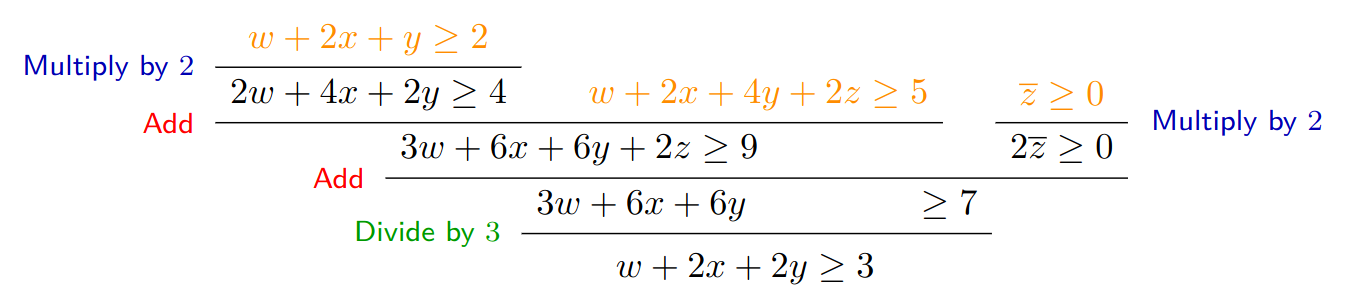
\includegraphics[scale=0.17]{_minted-cutting-planes-article/toy_example.png}

O leitor fica convidado a visitar o repositório público em \texttt{github.com/bernborgess/lean-cutting-planes}
e tentar por conta própria.


\section*{Conclusões}
% Capítulo de fechamento: conclusões e relação de trabalhos futuros.
Nós demonstramos a lógica de planos de corte como método correto para trabalhar com pseudo-booleanos.
Com nossa biblioteca \texttt{lean-cutting-planes} agora podemos utilizar o sistema de tipos de Lean
para validar com confiança passos dessa lógica. Com a documentação convidamos novos pesquisadores e
matemáticos a usar os resultados em verificadores.


% 6. Conclusion
% We have demonstrated Euclidean geometry as an attractive
% target for autoformalization. With our SMT-based symbolic
% engine, it is feasible to (1) automatically evaluate autofor-
% malized theorems statements and (2) have the model auto-
% formalize only explicit proof steps, leaving diagrammatic
% reasoning implicit. We have constructed the LeanEuclid
% benchmark to facilitate future research on autoformalizing
% Euclidean geometry.

\begin{thebibliography}{00}
    \bibitem{SatLive}       D. Le Berre, ``Sat Live! keep up to date with research on the satisfiability problem'', Acesso em http://www.satlive.org/.
    \bibitem{SatComp}       M. Heule, M. Jävisalo, M. Suda, ``The International SAT Competition Web Page'', Acesso em https://satcompetition.github.io/.
    \bibitem{CNF}           ``Conjunctive normal form'', Encyclopedia of Mathematics, EMS Press, 2001.
    \bibitem{PBSolve}       J. Nordström, ``Pseudo-Boolean Solving and Optimization'', Fevereiro de 2021.
    \bibitem{CutPlane}      J. Nordström, ``A Unified Proof System for Discrete Combinatorial Problems'', Novembro de 2023.
    \bibitem{LeanProver}    L. de Moura, S. Kong, J. Avigad, F. van Doorn, J. von Raumer ``The Lean Theorem Prover'', 25th International Conference on Automated Deduction (CADE-25), Berlin, Germany, 2015. Acesso em https://lean-lang.org/papers/system.pdf.
    \bibitem{Lean4}         L. de Moura, S. Ullrich ``The Lean 4 Theorem Prover and Programming Language'', 28th International Conference on Automated Deduction (CADE-28), Pittsburgh, USA, 2021. Acesso em https://lean-lang.org/papers/lean4.pdf.
    \bibitem{LTE}           J. Commelin, P. Scholze ``Liquid Tensor Experiment''. Acesso em https://math.commelin.net/files/LTE.pdf
    \bibitem{PFR}           T. Tao, ``The Polynomial Freiman-Ruzsa Conjecture'', Novembro de 2023. Acesso em https://teorth.github.io/pfr/.
    \bibitem{mathlib4}      The mathlib Community. 2020. ``The lean mathematical library''. In CPP 2020. 367-381. https://doi.org/10.1145/3372885.3373824
\end{thebibliography}

\newpage
\onecolumn
\appendix

\subsection{Definição de Inequações Pseudo-Booleanas}
\begin{minted}{lean4}
import Mathlib.Data.Fin.Tuple.Reflection

namespace PseudoBoolean

open FinVec BigOperators

abbrev Coeff (n : ℕ) := Fin n → (ℕ × ℕ)

def PBSum (cs : Coeff n) (xs : Fin n → Fin 2) :=
  ∑ i, let (p,n) := cs i;
    if xs i = 1 then p else n

def PBIneq (cs : Coeff n) (xs : Fin n → Fin 2) (const : ℕ) :=
  PBSum cs xs ≥ const

example : PBIneq ![(1,0)] ![1] 1 := by
  reduce                -- Expand the goal to 1 * 1 ≥ 1
  exact Nat.le_refl 1   -- Prove that 1 * 1 ≥ 1
  done

example : PBIneq ![(1,0),(2,0)] ![0,1] 2 := by
  reduce                -- Change goal to 1 * 0 + 2 * 1 ≥ 2
  exact Nat.le_refl 2   -- Prove 1 * 0 + 2 * 1 ≥ 2
  done

example : PBIneq ![(3,0),(4,0)] ![0,1] 2 := by
  reduce
  simp
  done

def mapBoth (f : α → β) (t : α × α) : β × β := Prod.map f f t

end PseudoBoolean
\end{minted}
\newpage

\subsection{Prova da Regra Multiplicação}
\begin{minted}{lean4}
import <<LeanCuttingPlanes>>.Basic

namespace PseudoBoolean

open BigOperators FinVec

theorem Multiplication
  {xs : Fin n → Fin 2}
  {as : Coeff n} {A : ℕ} (ha : PBIneq as xs A)
  (c : ℕ)
  : PBIneq (c • as) xs (c • A) := by
  unfold PBIneq PBSum at *
  simp only [Fin.isValue, ge_iff_le, nsmul_eq_smul, smul_eq_mul] at *
  apply nsmul_le_nsmul_right at ha
  specialize ha c
  rw [←Finset.sum_nsmul] at ha
  simp only [smul_eq_mul, Fin.isValue, mul_ite] at ha
  exact ha
  done

example
  (ha : PBIneq ![(1,0)] xs 3)
  : PBIneq ![(2,0)] xs 6 := by
  apply Multiplication ha 2
  done

end PseudoBoolean
\end{minted}
\newpage

\subsection{Prova da Regra Saturação}
\begin{minted}{lean4}
import <<LeanCuttingPlanes>>.Basic

namespace PseudoBoolean
open FinVec Matrix BigOperators Finset

-- @collares
lemma split_summation (n : ℕ) (as : Fin n → ℕ) (k : Fin n) :
    (∑i with i≠k, as i) + as k = (∑i, as i) := by
  have : (∑i with i=k, as i) = as k := by rw [Finset.sum_eq_single_of_mem] <;> simp
  rw [← this, ← Finset.sum_filter_add_sum_filter_not Finset.univ (· ≠ k)]
  simp only [ne_eq, Decidable.not_not]

lemma le_sum_min_of_le_sum {n A : ℕ} {as : Fin n → ℕ}
  (h : A ≤ ∑i, as i)
  : A ≤ ∑i, min A (as i) := by
  by_cases ha : ∀i, as i ≤ A
  . -- Assume all elements of as are ≤ A
    simp_rw [@Nat.min_eq_right A (as _) (ha _)]
    -- rewrite min A (as i) to (as i)
    exact h

  . -- Otherwise, ∃k, (as k) > A
    simp only [not_forall, not_le] at ha
    obtain ⟨k,hk⟩ := ha

    rw [←split_summation]
    -- Split goal from  ⊢ A ≤  ∑i, min A (as i)
    -- to               ⊢ A ≤ (∑i with i ≠ k, min A (as i)) + min A (as k)

    -- min A (as k) = A
    rw [min_eq_left_of_lt hk]

    -- ⊢ A ≤ (∑i,min A (as i) - A) + A
    exact Nat.le_add_left A _

theorem Saturation
  {xs : Fin n → Fin 2}
  {as : Coeff n} {A : ℕ} (ha : PBIneq as xs A)
  : PBIneq (map (mapBoth (min A)) as) xs A := by
  unfold PBIneq PBSum FinVec.map mapBoth at *
  simp only [Fin.isValue, ge_iff_le, Prod_map, seq_eq] at *
  have h := le_sum_min_of_le_sum ha
  simp_rw [apply_ite (min A) ((xs _ = 1)) ((as _).1) ((as _).2)] at h
  exact h
  done

example
  (ha : PBIneq ![(3,0),(4,0)] xs 3)
  : PBIneq ![(3,0),(3,0)] xs 3 := by
  apply Saturation ha
  done

end PseudoBoolean
\end{minted}
\newpage

\subsection{Prova da Regra Divisão}
\begin{minted}{lean4}
import <<LeanCuttingPlanes>>.Basic
import Mathlib.Algebra.Order.Floor.Div

namespace PseudoBoolean
open Finset FinVec BigOperators

def ceildiv (c : ℕ) (a : ℕ) := a ⌈/⌉ c

lemma ceildiv_le_ceildiv_right {a b : ℕ} (c : ℕ) (hab : a ≤ b)
  : a ⌈/⌉ c ≤ b ⌈/⌉ c := by
  repeat rw [Nat.ceilDiv_eq_add_pred_div]
  apply Nat.div_le_div_right
  apply Nat.sub_le_sub_right
  apply Nat.add_le_add_right
  exact hab
  done

-- @kbuzzard
theorem Nat.add_ceildiv_le_add_ceildiv (a b c : ℕ)
  : (a + b) ⌈/⌉ c ≤ (a ⌈/⌉ c) + (b ⌈/⌉ c) := by
  -- deal with c=0 separately
  obtain (rfl | hc) := Nat.eq_zero_or_pos c
  · simp
  -- 0 < c case
  -- First use the "Galois connection"
  rw [ceilDiv_le_iff_le_smul hc, smul_eq_mul]
  rw [mul_add]
  -- now use a standard fact
  gcongr <;> exact le_smul_ceilDiv hc
  done

-- @Ruben-VandeVelde
theorem Finset.ceildiv_le_ceildiv {α : Type*} (as : α → ℕ) (s : Finset α) (c : ℕ)
  : (∑i in s, as i) ⌈/⌉ c ≤ ∑i in s,(as i ⌈/⌉ c) := by
  classical
  induction s using Finset.cons_induction_on with
  | h₁ => simp
  | @h₂ a s ha ih =>
    rw [sum_cons, sum_cons]
    have h := Nat.add_ceildiv_le_add_ceildiv (as a) (∑x ∈ s, as x) c
    exact le_add_of_le_add_left h ih
    done

lemma ceildiv_ite (P : Prop) [Decidable P] (a b c : ℕ)
  : (if P then b else c) ⌈/⌉ a = if P then (b ⌈/⌉ a) else (c ⌈/⌉ a) := by
  split_ifs <;> rfl
  done







theorem Division
  {xs : Fin n → Fin 2}
  {as : Coeff n} {A : ℕ} (ha : PBIneq as xs A)
  (c : ℕ)
  : PBIneq (map (mapBoth (ceildiv c)) as) xs (ceildiv c A) := by
  unfold PBIneq PBSum ceildiv mapBoth at *
  simp only [Fin.isValue, ge_iff_le, gt_iff_lt,
             Prod_map, map_eq, Function.comp_apply] at *
  apply ceildiv_le_ceildiv_right c at ha
  apply le_trans ha
  simp only [←ceildiv_ite]
  apply Finset.ceildiv_le_ceildiv
  done

example
  (ha : PBIneq ![(3,0),(4,0)] xs 3)
  : PBIneq ![(2,0),(2,0)] xs 2 := by
  apply Division ha 2
  done

end PseudoBoolean

\end{minted}
\newpage

\subsection{Prova da Regra Adição}
\begin{minted}{lean4}
import <<LeanCuttingPlanes>>.Basic

namespace PseudoBoolean

open BigOperators FinVec Matrix

theorem Addition'
  (xs : Fin n → Fin 2)
  (as : Coeff n) (A : ℕ) (ha : PBIneq as xs A)
  (bs : Coeff n) (B : ℕ) (hb : PBIneq bs xs B)
  : PBIneq (as + bs) xs (A + B) := by
  unfold PBIneq PBSum at *
  simp only [Fin.isValue, ge_iff_le] at *
  simp_rw [←ite_add_ite]
  rw [Finset.sum_add_distrib]
  exact Nat.add_le_add ha hb
  done

def ReductionProp
  (xs : Fin n → Fin 2) (ks : Coeff n) (K : ℕ)
  : Prop :=
  let pos := λ i => ks i |>.1
  let neg := λ i => ks i |>.2
  let slack := (∑i, min (pos i) (neg i))
  let rs := λ i => (pos i - neg i,neg i - pos i)
  PBIneq rs xs (K - slack)

lemma ite_eq_bmul (x y : ℕ) (b : Fin 2)
  : (if b = 1 then x else y) = (x * b + y * (1 - b)) := by
  by_cases h : b = 0
  . rw [h]
    rw [if_neg]
    . simp only [Fin.isValue, Fin.val_zero, mul_zero, tsub_zero, mul_one, zero_add]
    trivial
  . -- b = 1
    apply Fin.eq_one_of_neq_zero b at h
    rw [h]
    simp only [Fin.isValue, ↓reduceIte, Fin.val_one, mul_one, ge_iff_le, le_refl,
      tsub_eq_zero_of_le, mul_zero, add_zero]

lemma reduce_terms (p n : ℕ) (x : Fin 2)
  : p * x + n * (1 - x) = (p - n) * x + (n - p) * (1 - x) + min p n  := by
  by_cases h : x = 0
  . rw [h]
    simp only [Fin.isValue, Fin.val_zero, mul_zero, tsub_zero, mul_one, zero_add]
    rw [Nat.min_comm]
    exact Nat.sub_add_min_cancel n p |>.symm

  . -- x = 1
    apply Fin.eq_one_of_neq_zero x at h
    rw [h]
    simp only [Fin.isValue, Fin.val_one, mul_one, ge_iff_le,
                le_refl, tsub_eq_zero_of_le, mul_zero, add_zero]
    exact Nat.sub_add_min_cancel p n |>.symm

theorem Reduction
  (xs : Fin n → Fin 2)
  (ks : Coeff n) (K : ℕ) (ha : PBIneq ks xs K)
  : ReductionProp xs ks K := by
  unfold ReductionProp PBIneq PBSum at *
  simp only [Fin.isValue, ge_iff_le, tsub_le_iff_right] at *
  simp_rw [ite_eq_bmul] at *
  rw [←Finset.sum_add_distrib]
  simp_rw [←reduce_terms]
  exact ha
  done

def AdditionProp
  (xs : Fin n → Fin 2)
  (as : Coeff n) (A : ℕ)
  (bs : Coeff n) (B : ℕ)
  : Prop :=
  ReductionProp xs (as + bs) (A + B)

theorem Addition
  {xs : Fin n → Fin 2}
  {as : Coeff n} {A : ℕ} (ha : PBIneq as xs A)
  {bs : Coeff n} {B : ℕ} (hb : PBIneq bs xs B)
  : AdditionProp xs as A bs B := by
  have hk := Addition' xs as A ha bs B hb
  exact Reduction xs (as + bs) (A + B) hk
  done

example
  (ha : PBIneq ![(1,0),(0,0)] xs 1)
  (hb : PBIneq ![(1,0),(1,0)] xs 2)
  : PBIneq ![(2,0),(1,0)] xs 3 := by
  apply Addition ha hb
  done

-- Reduction happens automatically
example
  (ha : PBIneq ![(3,0),(0,0),(1,0)] xs 1)
  (hb : PBIneq ![(0,0),(2,0),(0,1)] xs 2)
  : PBIneq ![(3,0),(2,0),(0,0)] xs 2 := by
  apply Addition ha hb
  done

end PseudoBoolean

\end{minted}
\newpage

\subsection{Implementação do Exemplo}
\begin{minted}{lean4}
import <<LeanCuttingPlanes>>

open PseudoBoolean

example
  (xs : Fin 4 → Fin 2)
  (c1 : PBIneq ![(1,0),(2,0),(1,0),(0,0)] xs 2)
  (c2 : PBIneq ![(1,0),(2,0),(4,0),(2,0)] xs 5)
  (c3 : PBIneq ![(0,0),(0,0),(0,0),(0,1)] xs 0)
  : PBIneq ![(1,0),(2,0),(2,0),(0,0)] xs 3
  := by
  let t1 : PBIneq ![(2,0),(4,0),(2,0),(0,0)] xs 4  := by apply Multiplication c1 2
  let t2 : PBIneq ![(3,0),(6,0),(6,0),(2,0)] xs 9  := by apply Addition t1 c2
  let t3 : PBIneq ![(0,0),(0,0),(0,0),(0,2)] xs 0  := by apply Multiplication c3 2
  let t4 : PBIneq ![(3,0),(6,0),(6,0),(0,0)] xs 7  := by apply Addition t2 t3
  exact Division t4 3
  done
\end{minted}


\end{document}
